%%%%%%%%%%%%%%%%%%%%%%%%%%%%%%%%%%%%%%%%%%%%%%%%%%%%%%%%%%%%%%%%%%%%%%%%%%%%%%%%
%
% \chapter{Introduction}\label{chIntroduction}
%
%%%%%%%%%%%%%%%%%%%%%%%%%%%%%%%%%%%%%%%%%%%%%%%%%%%%%%%%%%%%%%%%%%%%%%%%%%%%%%%%

ERMES (\underline{E}lectric \underline{R}egularized \underline{M}axwell's \underline{E}quations with \underline{S}ingularities) is an open-source software which solves the Maxwell's equations in frequency domain with the Finite Element Method (FEM). The new ERMES version 20.0 presented in this document is an upgrade of the ERMES version 7.0 presented in \cite{ERMES-CPC}. New features, modules, and FEM formulations have been implemented inside ERMES 20.0 to deal with the challenging problems usually found in the design and analysis of nuclear fusion reactors \cite{NAFEMS-CEM}. 

ERMES 20.0 is available for Windows and Linux systems and it has improved its capabilities to solve large problems on High Performance Computing (HPC) infrastructures thanks to its new interface with the solver libraries PETSc \cite{PETScWeb} and Python NumPy \cite{NumPyWeb}. As in previous versions, ERMES 20.0 features a graphical user-friendly interface integrated into the pre- and post- processor GiD \cite{GiDWeb}. GiD handles geometrical modelling, data input, meshing, and result visualization. ERMES 20.0 is licensed under the open-source software 2-clause BSD license and it is freely available to download on the developer's website \cite{ROtinWeb}.

New FEM formulations has been added to the regularized Maxwell's equations method already present in the previous versions \cite{EMPaper-Me, WRME-Performance}. These new additions are: the double-curl edge element formulation \cite{Jin}, and a local $L^{2}$ projection method with nodal and bubble elements \cite{L2P-BE}. For all the formulations, an $\textbf{A}-\phi$ potentials version has been included and, also stabilization terms with Lagrange multipliers which can be switched on and off (see Appendix \ref{chFEMForms} for details). The ample set of methods available in ERMES 20.0 allows the user to select the most suitable and stable formulation for each situation and generate the best possible conditioned matrix for each problem. These matrices can usually be solved efficiently with low-memory consuming iterative methods. 

ERMES 20.0 operates in the static, quasi-static and the high-frequency regimes, making it a versatile tool which can be used in a wide variety of situations. For instance, it had been applied to microwave engineering \cite{EMPaper-Me}, bioelectromagnetics \cite{NextGEM, ERMES-SAR-PIER, RFID-PIER}, electromagnetic compatibility \cite{Zt-IE3, Zt-CPC}, and electromagnetic forming \cite{LorentzForceFD, EMF-IJSS}. Now, thanks to the new electrostatic and cold plasma modules, the range of applications has been extended to relevant nuclear fusion engineering problems as: the computation of induced forces, plasma control, probability estimation of electric arc initiation, current distribution in arbitrary geometries, and the study of electromagnetic wave-plasma-wall interactions inside a fusion reactor \cite{NAFEMS-CEM, FWRF-AIP, APS-DPP-2023, APS-DPP-2022, STEP-Control}. 

\section{User interface}\label{ssUserInterface}

ERMES 20.0 has a Graphical User Interface (GUI) based on GiD \cite{GiDWeb}, which is an universal, adaptive and user-friendly tool for geometrical modelling, data input and visualization of results. GiD can be customized for being used with all types of numerical simulation programs. ERMES 20.0 uses GiD to create or import geometries, apply boundary conditions to surfaces, apply materials to volumes, set problem parameters, mesh, and visualize results. ERMES 20.0 interface is included in the problemtype folder \path{\ERMES_20.0}. ERMES-GiD workflow is as follows:\\ 
\quad\\
In GiD pre-processor, the user:
\begin{enumerate}
	\itemsep0em 
	\item Creates a geometry on GiD or imports it from another CAD program,
	\item Applies materials and boundary conditions on the CAD geometry,
	\item Sets problem parameters (e.g., FEM formulation, frequency, solver type),
	\item Generates a mesh clicking on the \textit{Mesh} button, 
	\item Clicks on the \textit{Calculate} button, and finally,
	\item GiD writes and saves ERMES 20.0 input files on the problem folder \ref{sERMESInputFiles}.
\end{enumerate}
ERMES 20.0 is called from the GiD pre-processor, and then ERMES 20.0:
\begin{enumerate}
    \itemsep0em 
	\item Reads the input files saved on the problem folder,
	\item Calculates, and
	\item Writes the results file on the problem folder.
\end{enumerate}
In GiD post-processor, the user:
\begin{enumerate}
	\itemsep0em 
	\item Opens ERMES 20.0 results file, and
	\item Visualizes and analyses the results.
\end{enumerate}

GiD simplifies the process of problem preparation and results visualization and it is the recommended pre- and post- processor tool for ERMES 20.0. Nevertheless, it is also possible to use a different pre- and post- processor software. 

If a pre-processor different from GiD is preferred, the only essential condition is to write the input files of ERMES 20.0 in the same format as stated in the \path{.bas} templates \ref{ssTemplateFiles}. These templates can be found in the GiD problem-type folder \path{\ERMES_20.0\ERMES.gid}. The \path{.bas} templates get the information from GiD and write the input files \path{.dat} in the format required by ERMES \ref{ssProblemFiles}. The input files \path{.dat} can be edited before calling ERMES 20.0 without having to use or opening GiD, which is also very useful for parametric batch calculations. In the GiD problemtype folder \path{\ERMES_20.0\Documents}, there are several batch and Python scripting examples that can be useful for automating tasks.

If a post-processor different from GiD is preferred, ERMES 20.0 can generate results files with different formats that can be edited to meet the needs of any other post-processor.

\section{C++ source code}

The ERMES 20.0 C++ source code, required external libraries, and license information are inside the folder \path{\ERMES_CPP_20.0} organized in eight different subfolders as described in the following:
\begin{enumerate}
	\itemsep0em 
	\item \textbf{\path{\ERMES}}: contains the finite element formulations, boundary conditions, and source elements. This folder also contains Gaussian integral tables and functions to write and read external files.
	
	\item \textbf{\path{\external_libraries}}: includes the libraries boost, gidpost, and dirent. It also contains the software required to generate Linux makefiles from a Microsoft Visual Studio 2022 solution in the folder \path{\cbp2make}, and the programs required to generate the files \path{input_c_parser.cpp} and \path{input_c_scanner.cpp} from the template scripts \path{input_c_parser.y} and \path{input_c_scanner.l} in the folder\path{\flex++bison++}.
	
	\item \textbf{\path{\includes}}: contains all the C++ objects template definitions and header files.
	
	\item \textbf{\path{\license}}: contains the details of the ERMES 20.0 open-source license.
	
	\item \textbf{\path{\linear_solvers}}: houses the internal iterative linear solvers used by ERMES 20.0.
	
	\item \textbf{\path{\sources}}: contains the main C++ objects of ERMES 20.0. The file \path{modeler.cpp} is where the solving strategies are implemented, the system matrix is build, discontinuities and singularities are treated and the geometrical normals are calculated. The file \path{kernel.cpp} connects the input data with the objects implemented in \path{modeler.cpp}. The files \path{input_c_parser.cpp} and \path{input_c_scanner.cpp} read the input files generated by the GiD pre-processor and give the data to the C++ objects implemented in \path{kernel.cpp} and \path{modeler.cpp}. The files \path{input_c_parser.cpp} and \path{input_c_scanner.cpp} are automatically generated with the programs flex++ and bison++ using the scripts \path{input_c_parser.y} and \path{input_c_scanner.l} as templates. Follow the steps given in \path{\external_libraries\flex++bison++\README.txt} to generate and include \path{input_c_parser.cpp} and \path{input_c_scanner.cpp} in ERMES 20.0. The file \path{gid_output.cpp} writes the calculated results in GiD post-processor format. The file \path{gid_output.cpp} uses the gidpost library located in \path{\external_libraries\gidpost}.
	
	\item \textbf{\path{\unix}}: includes the scripts required to compile ERMES 20.0 for Linux.
	
	\item \textbf{\path{\windows}}: contains the scripts required to compile ERMES 20.0 for Windows.
\end{enumerate}
Microsoft Visual Studio 2022 \cite{MVSWeb}, which is free for open-source code development, is the recommended tool to compile ERMES 20.0 for Windows and to navigate its source code. Open the file \path{\windows\ERMES.sln} with Microsoft Visual Studio 2022 to read the source code, load project settings, and set compiler configuration parameters. The current ERMES 20.0 project configuration parameters are shown in the Microsoft Visual Studio 2022 window of Figure \ref{VCConf}. Further instructions to compile for Windows can be found in the file \path{\windows\README.txt}.

To compile ERMES 20.0 for Linux, simply type the command \textit{make} in a Linux console inside the folder \path{\unix}. Further instructions for Linux compilation and how to generate the \path{makefile} can be found in \path{\unix\README.txt}.

\begin{figure}
	\begin{center}
		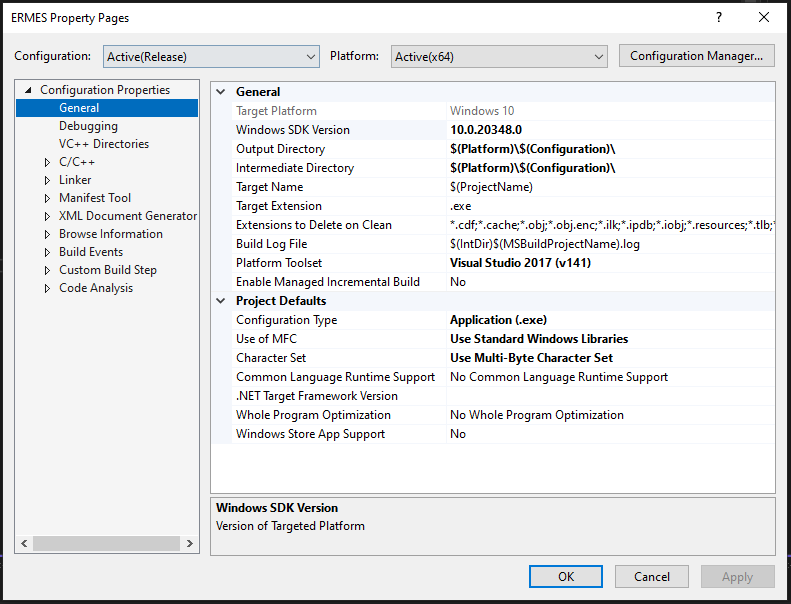
\includegraphics[width=\textwidth]{Contents/Figures/VC-Configuration.png}
		\caption{Microsoft Visual Studio 2022 project properties window for ERMES 20.0.}\label{VCConf}
	\end{center}
\end{figure}

\section{License}\label{License}

ERMES 20.0 source code, binary files and interface are under the following open-source 2-clause BSD license:\\
\\
\textit{Copyright (c) 2013 Ruben Otin, CIMNE (International Center for Numerical Methods in Engineering). All rights reserved.}\\
\\
\textit{Redistribution and use in source and binary forms, with or without modification, are permitted provided that the following conditions are met:}\\
\\
\textit{1. Redistributions of source code must retain the above copyright notice, this list of conditions and the following disclaimer.}\\
\\
\textit{2. Redistributions in binary form must reproduce the above copyright notice, this list of conditions and the following disclaimer in the documentation and/or other materials provided with the distribution.}\\
\\
\textit{This software is provided by the copyright holders and contributors "as is" and any express or implied warranties, including, but not limited to, the implied warranties of merchantability and fitness for a particular purpose are disclaimed. In no event shall the copyright holder or contributors be liable for any direct, indirect, incidental, special, exemplary, or consequential damages (including, but not limited to, procurement of substitute goods or services; loss of use, data, or profits; or business interruption) however caused and on any theory of liability, whether in contract, strict liability, or tort (including negligence or otherwise) arising in any way out of the use of this software, even if advised of the possibility of such damage.}








